\documentclass[../_main/handlingar.tex]{subfiles}

\begin{document}
\motion{Utskottstack i form av märken}
Hårda tider kräver hårda metoder. Endast en person inom phøset har ett accepterbart skägg inom årets
NollU. Detta behöver återgärdas genast. 

\begin{center}
	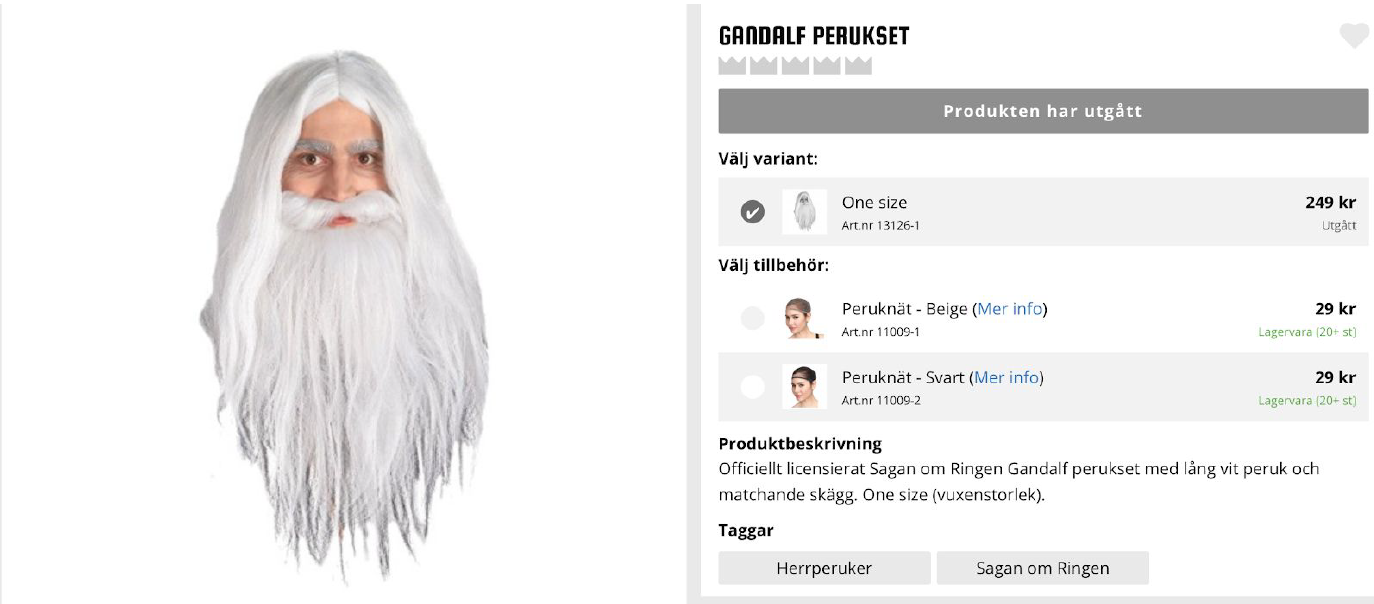
\includegraphics[width=12cm,height=6cm]{skagg.PNG}
\end{center}

Därför yrkar jag på
\begin{attsatser}
	\att köpa in nio godtyckliga perukset till en kostnad av \SI{2700}{kr},
	\att perukseten måste bäras av alla inom phøsgruppen inklusive øgp,
	\att peruksetet endast får tas av efter godkänd skäggväxt från 9 av 10 styrelsemedlemmar.
\end{attsatser}

\begin{signatures}{1}
	\mvh
	\signature{Anonym}{Skäggexpert}
\end{signatures}

\end{document}
